\section{Theorie}
  \subsection{Aufbau des Geiger-Müller-Zählrohres}
    Das Geiger-Müller-Zählrohr besteht aus einem Zylinder, der mit einer Spannungsquelle als
    Kathode dient. In der Achse des Zylinders befindet sich der Anodendraht, der ebenfalls an die
    Spannungsquelle angeschlossen ist. Im Inneren des Zylinders befindet sich ein Gasgemisch,
    im vorliegenden Versuch wird Argon und Ethylalkohol verwendet.
    \begin{figure}
      \centering
        \label{fig:aufbau1}
        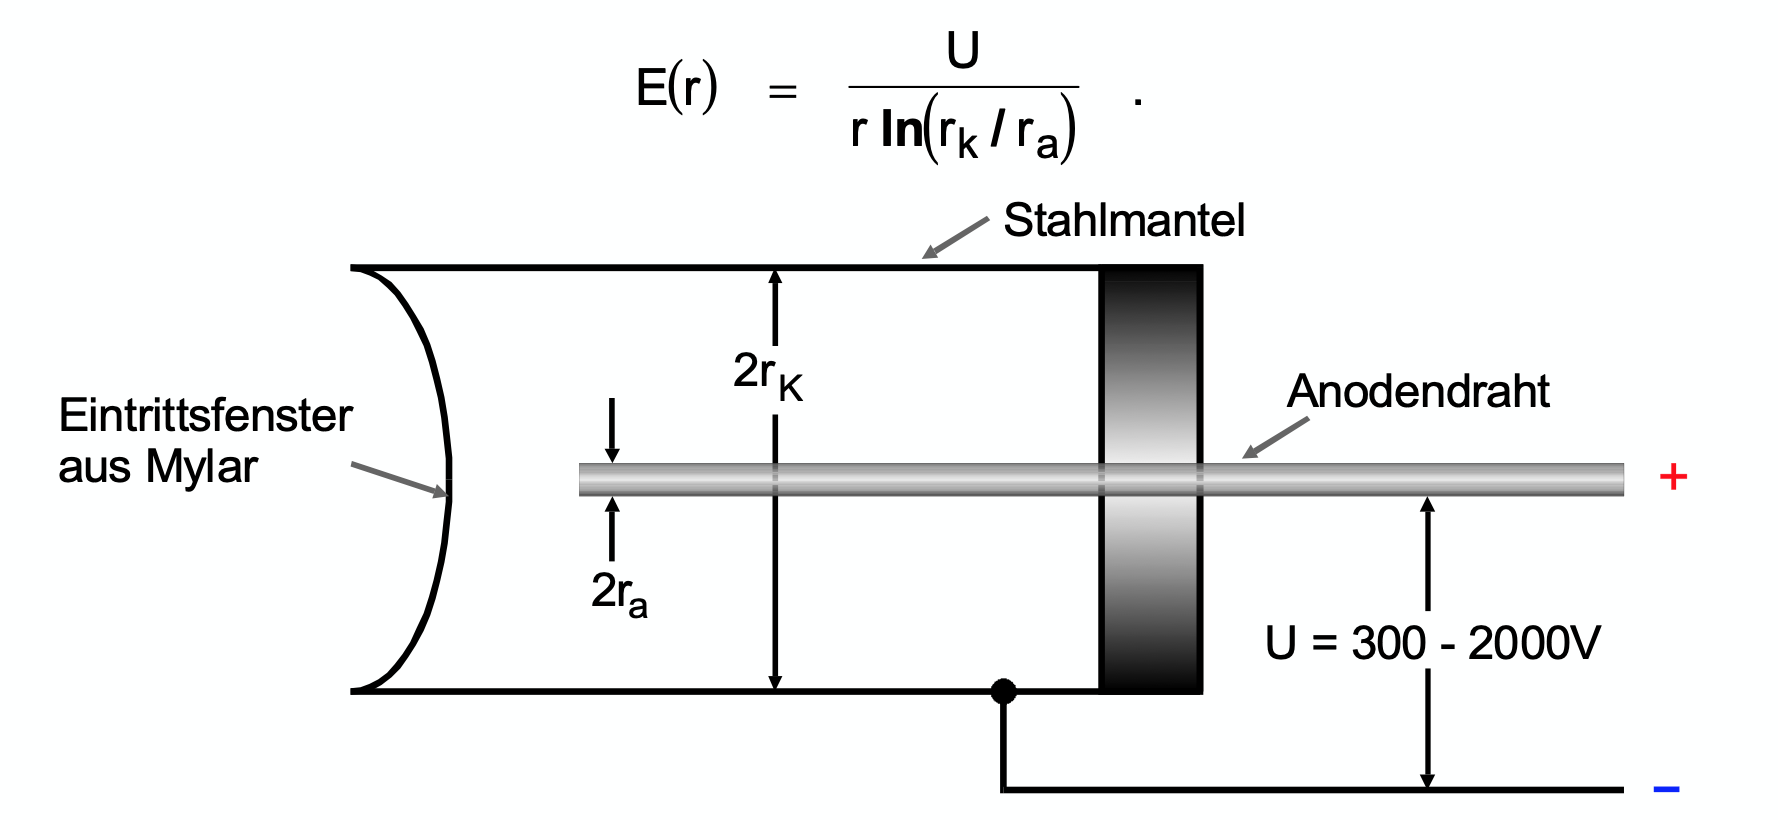
\includegraphics[scale=0.3]{content/AufbauGMZ.png}
        \caption{Der Aufbau eines Zählrohres mit Eintrittsfenster.}
    \end{figure}
    \\
    In obiger Abbildung ist ein Zählrohr mit Eintrittsfenster dargestellt. Dies wird benötigt,
    um einerseits das Gasgemisch innerhalb des Zylinders zu halten und andererseits den
    $\alpha$- und $\beta$-Teilchen zu ermöglichen, in den Zylinder zu gelangen. Es gibt auch
    Varianten des Zählrohres mit geschlossenem Metallzylinder, diese sind jedoch nicht in der Lage
    $\alpha$- und $\beta$-Teilchen zu messen und detektieren nur $\gamma$-Teilchen, da diese durch das
    Metall hindurch gelangen können.
    Durch Anlegen der Spannung bildet sich zwischen Anodendraht und Kathodenzylinder ein elektrisches
    radialsymmetrisches Feld aus. Die Feldstärke ist in Abbildung \ref{fig:aufbau1} ebenfalls
    angegeben. Wenn nun ein geladenes Teilchen in das Zählrohr gelangt, wird es durch Ionisationsakte
    seine Energie abgeben. Dadurch entstehen Ionen und Elektronen. Die Anzahl der positiven Ionen ist
    proportional zu der Energie des eingefallenen Teilchens. Dieser Prozess wird als Primärentladung
    bezeichnet.
    \begin{figure}
      \centering
        \label{fig:aufbau2}
        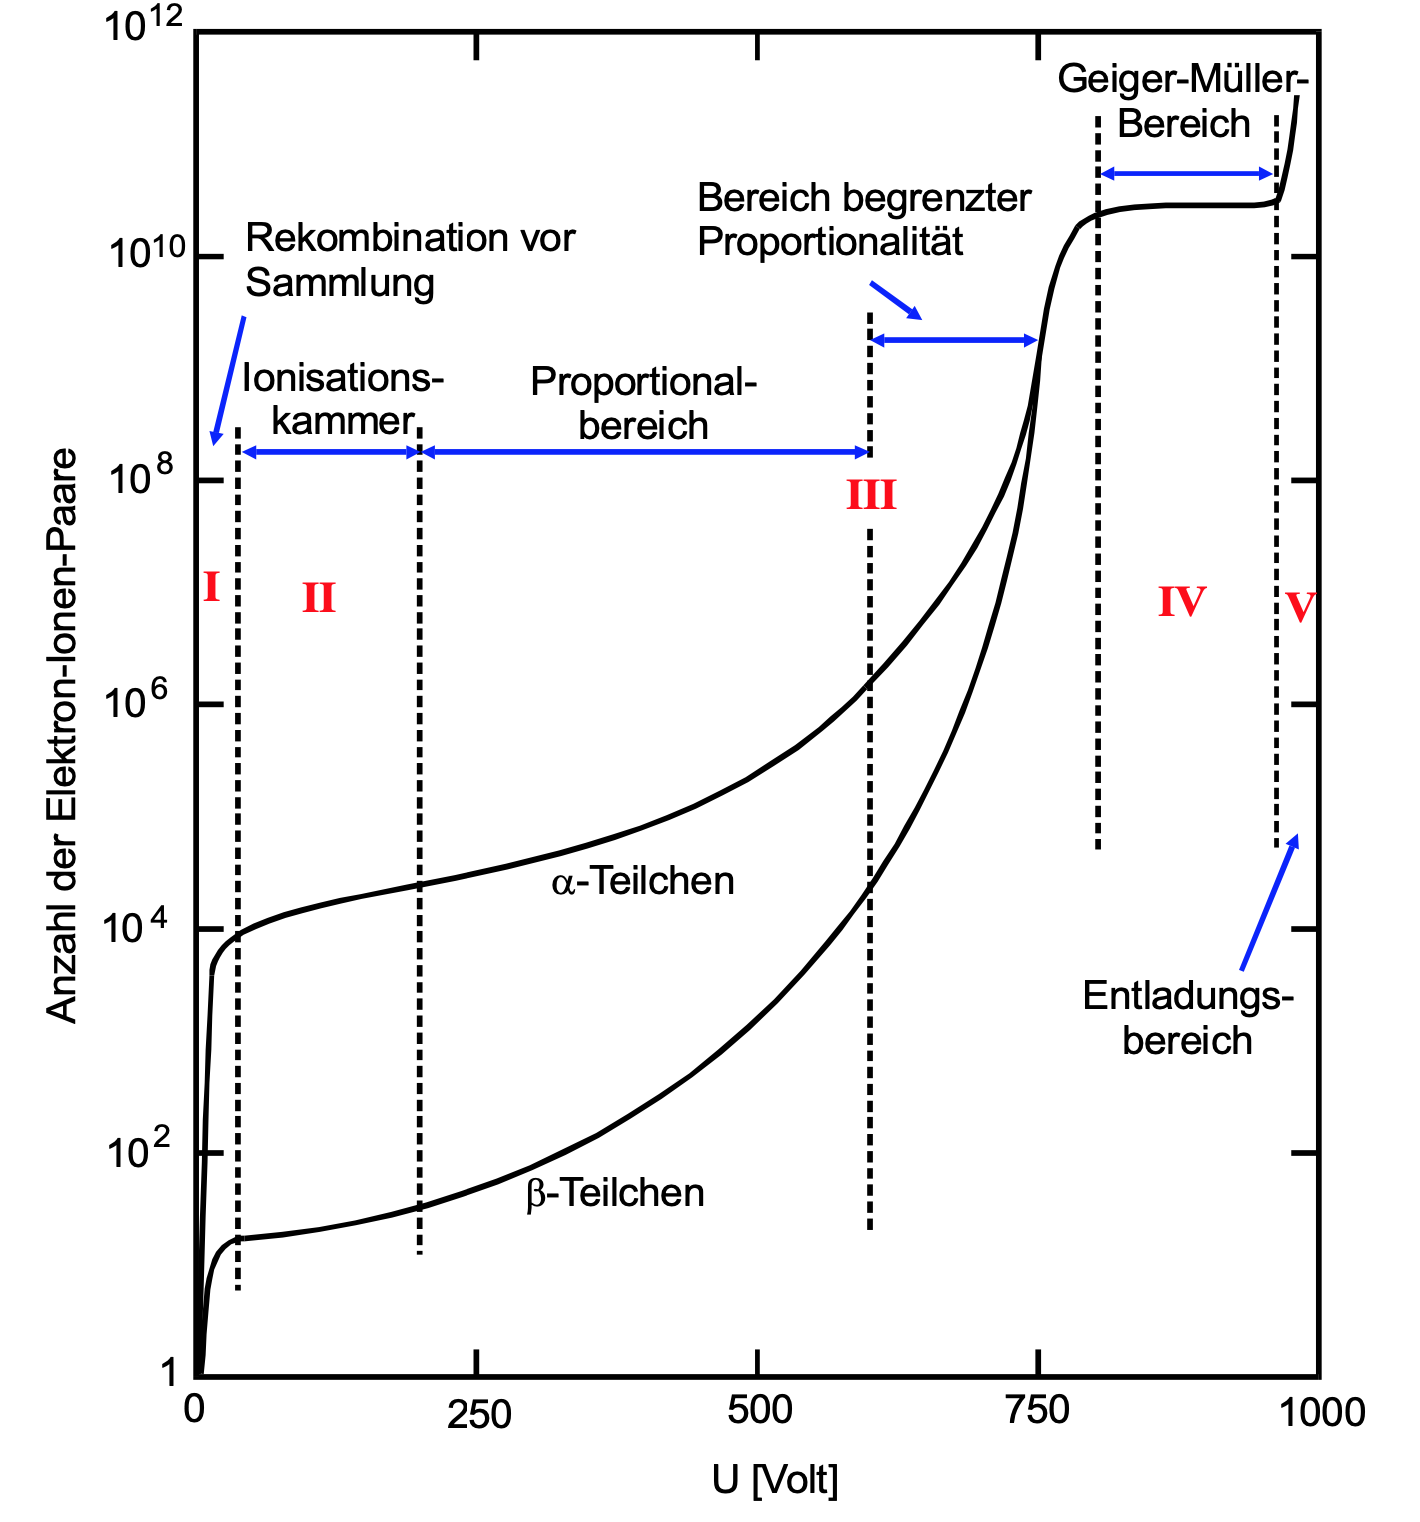
\includegraphics[scale=0.3]{content/SpannungAnzahlElektronenGMZ.png}
        \caption{Die Anzahl der erzeugten Elektronen-Ionenpaare aufgetragen gegen die Spannung.}
    \end{figure}
    \\
    In Abbildung \ref{fig:aufbau2} ist erkennbar, dass die Anzahl der Elektronen-Ionen-Paare von der
    angelegten Spannung abhängt. Wenn die Spannung nicht hoch genug ist, erreichen nicht alle
    Elektronen die Anode und rekombinieren. Dies ist in Abbildung \ref{fig:aufbau2} der Bereich [1].
    Bei erhöhter Spannung steigt die Feldstärke soweit an, dass die Rekombinationswahrscheinlichkeit
    sehr gering wird. Der Ionisationsstrom ist nun proportional zu der Energie und der Intensität der
    einfallenden Teilchen, da fast alle Elektronen zu der Anode gelangen. Dies entspricht Bereich [2]
    in Abbildung \ref{fig:aufbau2}. Ein solches Gerät wird als Ionisationskammer bezeichnet.
    Da eine Ionisationskammer nur relativ geringe Ströme erzeugt, kann eine solche Apparatur nur bei
    hohen Intensitäten verwendet werden.
    Bei weiterer Erhöhung der Feldstärke erreichen die aus der Ionisation entstandenen Elektronen
    genug Energie um selber zu ionisieren. Dieser Prozess wird als Stoßionisation bezeichnet. Dadurch
    ergibt sich eine exponentielle Erzeugung von Elektronen, eine Townsend-Lawine. Die am Anodendraht
    gemessene Ladung $Q$ ist nun recht groß und daher gut messbar. Dieser Ladungsimpuls ist
    proportional zu der Energie und Intensität der einfallenden Teilchen und ermöglicht daher eine
    Bestimmung dieser Werte. Eine in diesem Spannungsbereich arbeitende Apparatur wird als
    Proportionalitätszählrohr bezeichnet und ist in Abbildung \ref{fig:aufbau2} Bereich [3]
    dargestellt.
    Noch höhere Spannung sorgt dafür dass die Ladung $Q$ unabhängig von der Primären Ionisation wird.
    Dieser Bereich heißt Auslösebereich und ist in Abbildung \ref{fig:aufbau2} als Bereich [4]
    dargestellt. Nun entstehen bei der Primären Ionisation neben den Ionen und Elektronen auch
    UV-Photonen durch Elektronenstoß der durch die höhere Spannung angeregten Argon-Atomen. Die
    UV-Photonen sind Ladungsneutral und können sich daher auch senkrecht zum elektrischen Feld bewegen.
    Dadurch setzt sich die Lawine im gesamten Volumen des Zählrohrs fort. In diesem Spannungsbereich
    kann nur die Intensität gemessen werden.
  \subsection{Die Totzeit}
    Nachdem ein Teilchen eingetroffen ist, bewegen sich die abgespaltenen Elektronen recht schnell zu
    dem Anodendraht. Die Ionen besitzen eine wesentlich größere Masse und brauchen daher länger um zu
    der Kathode zu gelangen. Sie bauen eine kurzfristige, radialsymmetrische, positive Raumladung auf,
    wodurch die Feldstärke soweit gesenkt wird, dass keine weitere Stoßionisation möglich ist und
    daher auch keine weiteren Teilchen detektiert werden können. Die Zeit, in der keine Teilchen
    registriert werden können, wird Totzeit $T$ genannt. Die Ionen bewegen sich langsam auf die
    Kathode zu, was zum Abbau der Raumladung und Anstieg der Feldstärke führt. Die Stoßionisierung
    wird wieder möglich und das Zählrohr ist wieder dazu in der Lage, einfallende Teilchen zu
    registrieren. Bis zur vollständigen Neutralisation der Ionen sind die Ladungsimpulse geringer.
    Dies wird mit Erholungszeit $T_{E}$ bezeichnet.
  \subsection{Die Nachentladung}
    Die Ionen besitzen genug Energie, um aus dem Kathodenzylinder Elektronen abzuspalten. Die auf
    diese Weise aus dem Metall abgespaltenen Elektronen nennt man Sekundärelektronen. Sie können
    ebenfalls das Zählrohr auslösen. Diese Nachentladungen führen dazu, das ein Teilchen mehrere
    Ladungsimpulse zur Folge hat und damit das Registrieren der Teilchen unmöglich wird. Man kann
    diesen Vorgang verhindern, indem zu dem Gasgemisch Alkoholdämpfe hinzugefügt werden. Die Ionen
    kollidieren auf dem Weg zu der Kathodenwand mit den Alkoholmolekülen und werden von den Edelgasen
    ionisiert. Bei dem auftreffen der Alkoholmoleküle an der Kathodenwand werden keine Elektronen frei,
    da die Energie zur Anregung einer Schwingung der vielatomigen Alkoholmoleküle verbraucht wird.
    Das Zählrohr registriert daher nur die einfallenden Teilchen.
\label{sec:Theorie}
